\documentclass[11pt,a4paper]{article}

\usepackage[utf8]{inputenc}
\usepackage[T1]{fontenc}
\usepackage[italian]{babel}
\usepackage{lmodern}
\usepackage[a4paper,margin=2.5cm]{geometry}
\usepackage{amsmath}
\usepackage{graphicx}
\usepackage{booktabs}
\usepackage{multirow}
\usepackage{float}
\usepackage[font=small,labelfont=bf]{caption}
\usepackage{parskip}
\usepackage[hidelinks]{hyperref}

\graphicspath{{figures/}}
\hypersetup{pdftitle={Facial Expression Recognition su FER-2013 - Gabriel Betti}}

\title{\textbf{Facial Expression Recognition su FER-2013:\\confronto tra HOG+SVM e CNN, failure modes e bias}}
\author{Gabriel Betti \\ Matricola 178267 \\ \href{mailto:betti.gabriel@spes.uniud.it}{betti.gabriel@spes.uniud.it}}
\date{\today}

\begin{document}
\maketitle

\begin{abstract}
Questo lavoro confronta una pipeline classica (descrittore HOG e SVM lineare) con reti convoluzionali per il riconoscimento di sette espressioni facciali sul dataset FER-2013 (volti $48\times48$ in scala di grigi). Il protocollo segue lo split ufficiale della competizione ICML 2013 (\textit{PublicTest} come validation, \textit{PrivateTest} come test) e rimuove dal training 703 immagini identiche a immagini di validation o test. Una rete residua leggera addestrata da zero (ResNet-Lite) raggiunge sul test un'accuratezza del $67.3\% \pm 0.2\%$ e una macro-F1 di $0.657$ (media su tre seed), contro il $40.6\%$ (macro-F1 $0.349$) di HOG+LinearSVC e il $63.2\%$ di MobileNetV2 in transfer learning. Un esperimento di ablation mostra che label smoothing e campionamento bilanciato migliorano la macro-F1 (da $0.636$ a $0.656$) e la recall della classe minoritaria \textit{Disgust}, senza un effetto significativo sull'accuratezza globale (test di McNemar, $p=0.35$). L'analisi degli errori evidenzia confusioni sistematiche tra \textit{Fear}, \textit{Sad}, \textit{Neutral} e \textit{Angry}, in parte riconducibili al rumore delle etichette. L'analisi per sottogruppi di luminosità, contrasto e nitidezza non rileva differenze statisticamente significative; le immagini più scure mostrano l'accuratezza più bassa, ma l'effetto è debole e in parte spiegato dalla diversa composizione delle classi.
\end{abstract}

\section{Introduzione}
Il riconoscimento automatico delle espressioni facciali (\textit{Facial Expression Recognition}, FER) consiste nell'assegnare a un'immagine di volto una tra un insieme di emozioni di base. FER-2013 \cite{goodfellow2015challenges} è uno dei benchmark più usati per questo compito ed è particolarmente difficile per tre motivi.

\begin{enumerate}
    \item \textbf{Bassa risoluzione.} Le immagini sono $48\times48$ pixel in scala di grigi: dettagli come la contrazione delle sopracciglia o la forma della bocca occupano pochi pixel.
    \item \textbf{Etichette rumorose.} Le immagini sono state raccolte dal web tramite parole chiave e filtrate da annotatori umani. L'accuratezza umana stimata è del $65\pm5\%$ \cite{goodfellow2015challenges}, e la successiva ri-annotazione con 10 annotatori per immagine (FER+) ha confermato che una parte delle etichette originali è ambigua o errata \cite{barsoum2016ferplus}.
    \item \textbf{Sbilanciamento.} \textit{Happy} rappresenta circa un quarto del training, mentre \textit{Disgust} meno dell'1.5\% (Tabella~\ref{tab:data}).
\end{enumerate}

Gli obiettivi del progetto sono: (i) implementare e confrontare una pipeline HOG+SVM e approcci basati su CNN; (ii) analizzare la confusione tra emozioni visivamente simili; (iii) studiare i bias del modello su sottogruppi del dataset; (iv) valutare l'effetto di strategie di mitigazione per rumore ed etichette sbilanciate (label smoothing, campionamento bilanciato, focal loss). Tutti gli esperimenti sono contenuti in un unico notebook eseguibile su Google Colab; risultati e figure riportati in questo documento sono generati da quel notebook.

\section{Stato dell'arte}
\paragraph{Approcci classici.} Prima del deep learning la FER si basava su descrittori progettati a mano, come gli istogrammi dei gradienti orientati (HOG) \cite{dalal2005hog} o i Local Binary Patterns, seguiti da classificatori come le SVM. Questi metodi sono leggeri e interpretabili, ma i descrittori sono fissi: non si adattano alle variazioni di posa, illuminazione e occlusione tipiche delle immagini raccolte ``in the wild''.

\paragraph{CNN su FER-2013.} Le varianti di CNN proposte in letteratura riportano su FER-2013 accuratezze comprese tra il 65\% e il 72.7\%; con una rete VGG e una ricerca accurata degli iperparametri si arriva al 73.28\% per una singola rete, senza dati aggiuntivi \cite{khaireddin2021fer}. Il fatto che questi valori superino la stima di accuratezza umana non implica overfitting: la stima umana del $65\pm5\%$ deriva da esperimenti su piccola scala \cite{goodfellow2015challenges}, mentre i modelli sono valutati su un test set separato.

\paragraph{Rumore, sbilanciamento e bias.} Per il rumore delle etichette sono comuni il \textit{label smoothing} \cite{szegedy2016rethinking} e l'uso di distribuzioni di etichette \cite{barsoum2016ferplus}. Per lo sbilanciamento si usano ripesatura della loss, campionamento bilanciato \cite{mahajan2018weakly} o la focal loss \cite{lin2017focal}. Sul piano dei bias, studi su dataset annotati con attributi demografici mostrano differenze di accuratezza tra gruppi di genere, età ed etnia \cite{xu2020bias}. FER-2013 non fornisce tali attributi.

\paragraph{Posizionamento.} Questo progetto non mira al record su FER-2013. L'obiettivo è un confronto controllato tra approcci, con un protocollo di valutazione pulito, stime di incertezza e un'analisi critica degli errori. Come riferimento, un risultato tra il 65\% e il 70\% è in linea con CNN addestrate da zero senza ensemble.

\section{Dataset e protocollo sperimentale}
\subsection{Split e pulizia dei dati}
Si usa la versione Kaggle di FER-2013 (\texttt{msambare/fer2013}), che contiene la cartella \texttt{train} (28\,709 immagini) e una cartella \texttt{test} che unisce i due test set ufficiali. Usando il prefisso del nome file si ricostruisce lo split originale: \textit{Training} per l'addestramento, \textit{PublicTest} (3\,589) come \textbf{validation} e \textit{PrivateTest} (3\,589) come \textbf{test}. La validation è usata per early stopping e scelta del modello; il test è usato una sola volta, nella valutazione finale.

Un audit basato sull'hash dei pixel ha rilevato 1\,516 gruppi di immagini identiche nel dataset, 57 dei quali con etichette diverse tra le copie (prova diretta del rumore di annotazione). Per evitare che il modello venga valutato su immagini già viste in training, sono state rimosse \textbf{703 immagini dal training} identiche a immagini di validation o test e \textbf{46 immagini dalla validation} identiche a immagini del test. La Tabella~\ref{tab:data} riporta la distribuzione finale.

\begin{table}[H]
\centering
\caption{Distribuzione delle classi dopo la rimozione dei duplicati tra split.}
\label{tab:data}
\begin{tabular}{lrrrr}
\toprule
Classe & Training & Validation & Test & \% training \\
\midrule
Angry    & 3\,879 & 461 & 491 & 13.9 \\
Disgust  &    389 &  55 &  55 &  1.4 \\
Fear     & 3\,988 & 494 & 528 & 14.2 \\
Happy    & 7\,157 & 890 & 879 & 25.6 \\
Neutral  & 4\,917 & 601 & 626 & 17.6 \\
Sad      & 4\,780 & 650 & 594 & 17.1 \\
Surprise & 2\,896 & 392 & 416 & 10.3 \\
\midrule
Totale   & 28\,006 & 3\,543 & 3\,589 & \\
\bottomrule
\end{tabular}
\end{table}

\subsection{Metriche e test statistici}
Oltre all'accuratezza si riporta la \textbf{macro-F1}, media non pesata delle F1 per classe: con classi sbilanciate l'accuratezza premia le classi frequenti, mentre la macro-F1 dà lo stesso peso a \textit{Disgust} e \textit{Happy}. La macro-F1 sulla validation è il criterio di selezione di tutti i modelli. Per ogni metrica sul test si calcola un intervallo di confidenza al 95\% con bootstrap (1\,000 ricampionamenti del test set). Le differenze tra due modelli sono verificate con il test di McNemar esatto \cite{dietterich1998tests}, che confronta le immagini classificate correttamente da un solo dei due modelli.

\subsection{Riproducibilità}
Tutti i seed (Python, NumPy, TensorFlow) sono fissati e le operazioni di TensorFlow sono rese deterministiche. Gli esperimenti sono stati eseguiti su Google Colab con GPU NVIDIA T4, TensorFlow 2.21, Keras 3.13 e scikit-learn 1.6, in precisione mista. Ogni esperimento salva su disco pesi, curve di training, predizioni e metriche; il file \texttt{results.json} raccoglie tutti i valori riportati in questo documento.

\section{Pipeline e scelte progettuali}
\subsection{Baseline classica: HOG + LinearSVC}
Da ogni immagine si estrae un descrittore HOG \cite{dalal2005hog} con 9 orientazioni, celle $8\times8$ e blocchi $2\times2$ con normalizzazione L2-Hys (900 dimensioni). Il classificatore è una SVM lineare (implementazione LIBLINEAR di scikit-learn) con pesi di classe inversamente proporzionali alla frequenza. Il parametro $C\in\{0.01, 0.1, 1\}$ è scelto sulla validation ($C=1$). La scelta di un kernel lineare è dettata dal costo: con circa 28\,000 esempi un kernel RBF richiederebbe un tempo di addestramento molto superiore.

\subsection{CNN addestrata da zero: ResNet-Lite}
La rete principale è una CNN residua compatta (5.0 milioni di parametri): una convoluzione iniziale a 64 filtri seguita da quattro blocchi residui \cite{he2016resnet} con 64, 128, 256 e 512 filtri. Ogni blocco contiene due convoluzioni $3\times3$ con Batch Normalization e una connessione residua; dopo ogni blocco seguono max pooling e dropout crescente (da 0.2 a 0.4). La testa è composta da global average pooling, uno strato denso da 256 unità e dropout 0.5.

Le motivazioni sono tre. Le connessioni residue rendono stabile l'addestramento di una rete con 9 strati convoluzionali. Il global average pooling riduce drasticamente i parametri della testa rispetto a un \texttt{Flatten}, limitando l'overfitting. Una rete di questa taglia si addestra in circa 28 minuti su una GPU gratuita, il che rende possibili ablation e ripetizioni su più seed.

\textbf{Data augmentation} (solo in training): flip orizzontale, rotazione casuale fino a $\pm18^\circ$, traslazione e zoom fino al 5\%, variazione di contrasto fino al 15\%. Trasformazioni geometriche più ampie su immagini $48\times48$ rischiano di tagliare bocca e sopracciglia, cioè le regioni più informative.

\textbf{Ottimizzazione}: AdamW con weight decay $10^{-4}$, learning rate iniziale $10^{-3}$ con decadimento a coseno su 50 epoche, batch di 64 immagini. Si conservano i pesi dell'epoca con la migliore macro-F1 sulla validation (early stopping con pazienza 10). Con il decadimento a coseno il learning rate tende a zero alla fine dell'addestramento, per cui è atteso che l'epoca migliore cada nelle ultime epoche.

\subsection{Strategie di mitigazione}
Per isolare l'effetto delle mitigazioni la stessa rete è stata addestrata in tre configurazioni:
\begin{itemize}
    \item \textbf{A -- baseline}: cross-entropy, campionamento naturale, nessuna mitigazione.
    \item \textbf{B -- label smoothing + balanced sampling}: cross-entropy con label smoothing 0.1 \cite{szegedy2016rethinking}, che riduce la sicurezza del modello sulle etichette (un effetto desiderabile quando le etichette sono rumorose); ogni batch viene estratto con probabilità di classe proporzionale alla radice quadrata della frequenza (\textit{square-root sampling} \cite{mahajan2018weakly}). Con questa scelta la quota di \textit{Disgust} nei batch sale dall'1.4\% al 4.7\% e quella di \textit{Happy} scende dal 25.6\% al 20.0\%: le classi rare vengono viste più spesso senza replicare le stesse 389 immagini di \textit{Disgust} fino a memorizzarle, come avverrebbe con un campionamento uniforme.
    \item \textbf{C -- focal loss}: focal loss \cite{lin2017focal} con $\gamma=2$ e un peso $\alpha_k$ per ciascuna classe proporzionale a $1/\sqrt{n_k}$ (da 0.58 per \textit{Happy} a 2.50 per \textit{Disgust}), combinata con label smoothing 0.1 e campionamento naturale. La focal loss riduce il peso degli esempi già classificati con sicurezza e concentra l'addestramento su quelli difficili.
\end{itemize}

\subsection{Transfer learning: MobileNetV2}
Come confronto con una rete pre-addestrata si usa MobileNetV2 \cite{sandler2018mobilenetv2} con pesi pre-addestrati su ImageNet. L'immagine viene replicata su tre canali e ridimensionata a $96\times96$. L'addestramento avviene in due stadi: 5 epoche con il backbone congelato per addestrare la nuova testa, poi fine-tuning dei blocchi da \texttt{block\_9} in poi per un massimo di 25 epoche (learning rate $10^{-4}$ con decadimento a coseno). Le Batch Normalization del backbone restano congelate per non alterare le statistiche apprese su ImageNet. Augmentation e mitigazioni sono le stesse della configurazione selezionata (B).

\section{Risultati}
\subsection{Selezione del modello}
La Tabella~\ref{tab:val} riporta le metriche di validation. La configurazione B ottiene la macro-F1 più alta ed è stata scelta come modello finale; è stata poi riaddestrata con due seed aggiuntivi.

\begin{table}[H]
\centering
\caption{Risultati sulla validation (PublicTest). L'epoca è quella con la migliore macro-F1.}
\label{tab:val}
\begin{tabular}{llccc}
\toprule
Modello & Seed & Accuratezza & Macro-F1 & Epoca migliore \\
\midrule
HOG + LinearSVC ($C=1$) & -- & 40.53\% & 0.351 & -- \\
A -- baseline & 42 & 65.48\% & 0.622 & 45 \\
B -- LS + balanced sampling & 42 & 66.30\% & \textbf{0.642} & 47 \\
C -- focal loss & 42 & 65.34\% & 0.631 & 45 \\
B -- LS + balanced sampling & 43 & 66.41\% & 0.646 & 48 \\
B -- LS + balanced sampling & 44 & 66.30\% & 0.636 & 48 \\
MobileNetV2 & 42 & 61.90\% & 0.591 & 24 / 30 \\
\bottomrule
\end{tabular}
\end{table}

\begin{figure}[H]
\centering
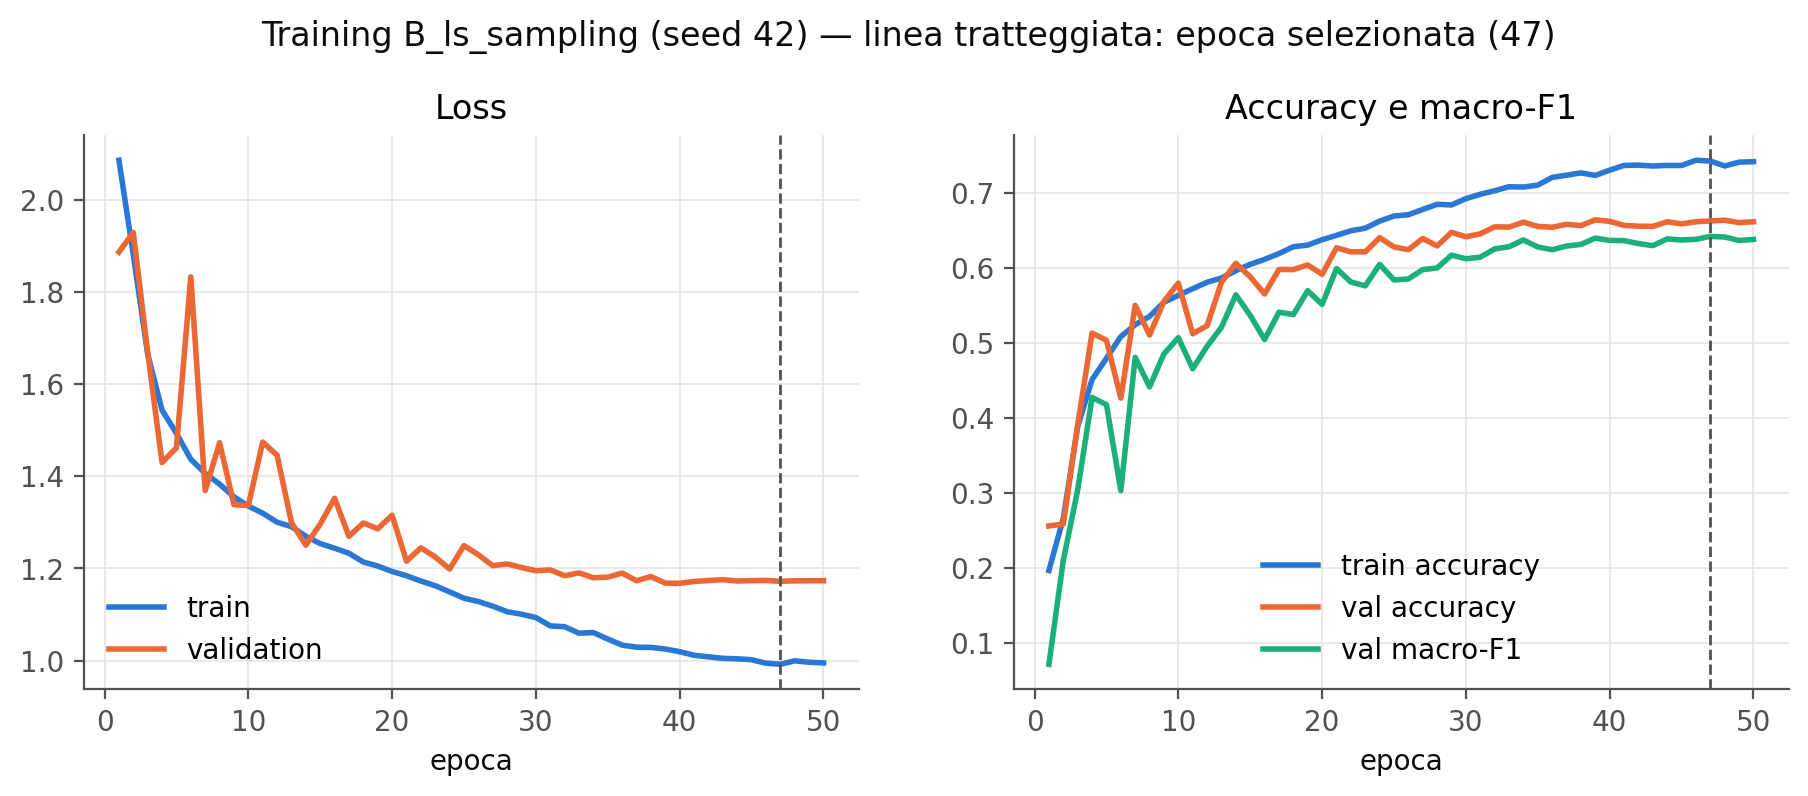
\includegraphics[width=\linewidth]{training_curves.png}
\caption{Curve di training del modello finale (B, seed 42). La distanza tra le curve di train e validation cresce dopo l'epoca 20 ma la loss di validation resta stabile: la regolarizzazione contiene l'overfitting.}
\label{fig:curves}
\end{figure}

\subsection{Valutazione sul test}
\begin{table}[H]
\centering
\caption{Risultati sul test (PrivateTest, 3\,589 immagini) con intervalli di confidenza bootstrap al 95\%.}
\label{tab:test}
\begin{tabular}{lcc}
\toprule
Modello & Accuratezza [IC 95\%] & Macro-F1 [IC 95\%] \\
\midrule
HOG + LinearSVC & 40.60\% [39.1, 42.2] & 0.349 [0.334, 0.364] \\
A -- baseline & 66.70\% [65.3, 68.1] & 0.636 [0.615, 0.655] \\
B -- LS + balanced sampling & 67.29\% [65.9, 68.9] & 0.656 [0.636, 0.676] \\
C -- focal loss & 67.40\% [66.0, 68.9] & 0.651 [0.631, 0.670] \\
MobileNetV2 & 63.22\% [61.6, 64.8] & 0.609 [0.587, 0.630] \\
\midrule
\textbf{B, media su 3 seed} & $\mathbf{67.32\% \pm 0.18}$ & $\mathbf{0.657 \pm 0.0004}$ \\
\bottomrule
\end{tabular}
\end{table}

Il modello finale è stabile rispetto al seed (accuratezze 67.29\%, 67.51\%, 67.15\%). I test di McNemar danno il seguente quadro:
\begin{itemize}
    \item \textbf{CNN vs HOG+SVM}: 1\,178 immagini corrette solo per la CNN contro 220 solo per la SVM ($p<10^{-150}$). Il vantaggio della CNN riguarda tutte le classi; solo per \textit{Disgust} la recall della SVM è vicina a quella delle CNN, ma con una precisione molto più bassa (Tabella~\ref{tab:recall}).
    \item \textbf{B vs MobileNetV2}: 461 contro 315 ($p=1.8\times10^{-7}$). La rete addestrata da zero è significativamente migliore.
    \item \textbf{B vs A}: 243 contro 222 ($p=0.35$). Le mitigazioni non cambiano in modo significativo l'accuratezza globale.
\end{itemize}

\subsection{Effetto delle mitigazioni}
\begin{table}[H]
\centering
\caption{Recall per classe sul test.}
\label{tab:recall}
\begin{tabular}{lccccccc}
\toprule
Modello & Angry & Disgust & Fear & Happy & Neutral & Sad & Surprise \\
\midrule
HOG + LinearSVC & 0.226 & 0.582 & 0.193 & 0.696 & 0.374 & 0.209 & 0.582 \\
A -- baseline & 0.540 & 0.509 & 0.441 & \textbf{0.879} & \textbf{0.728} & \textbf{0.591} & 0.692 \\
B -- LS + sampling & 0.558 & \textbf{0.636} & 0.462 & 0.861 & 0.722 & 0.577 & 0.745 \\
C -- focal loss & \textbf{0.595} & 0.618 & 0.443 & 0.856 & 0.716 & 0.582 & \textbf{0.752} \\
MobileNetV2 & 0.544 & 0.545 & \textbf{0.475} & 0.833 & 0.692 & 0.434 & 0.716 \\
\bottomrule
\end{tabular}
\end{table}

\begin{figure}[H]
\centering
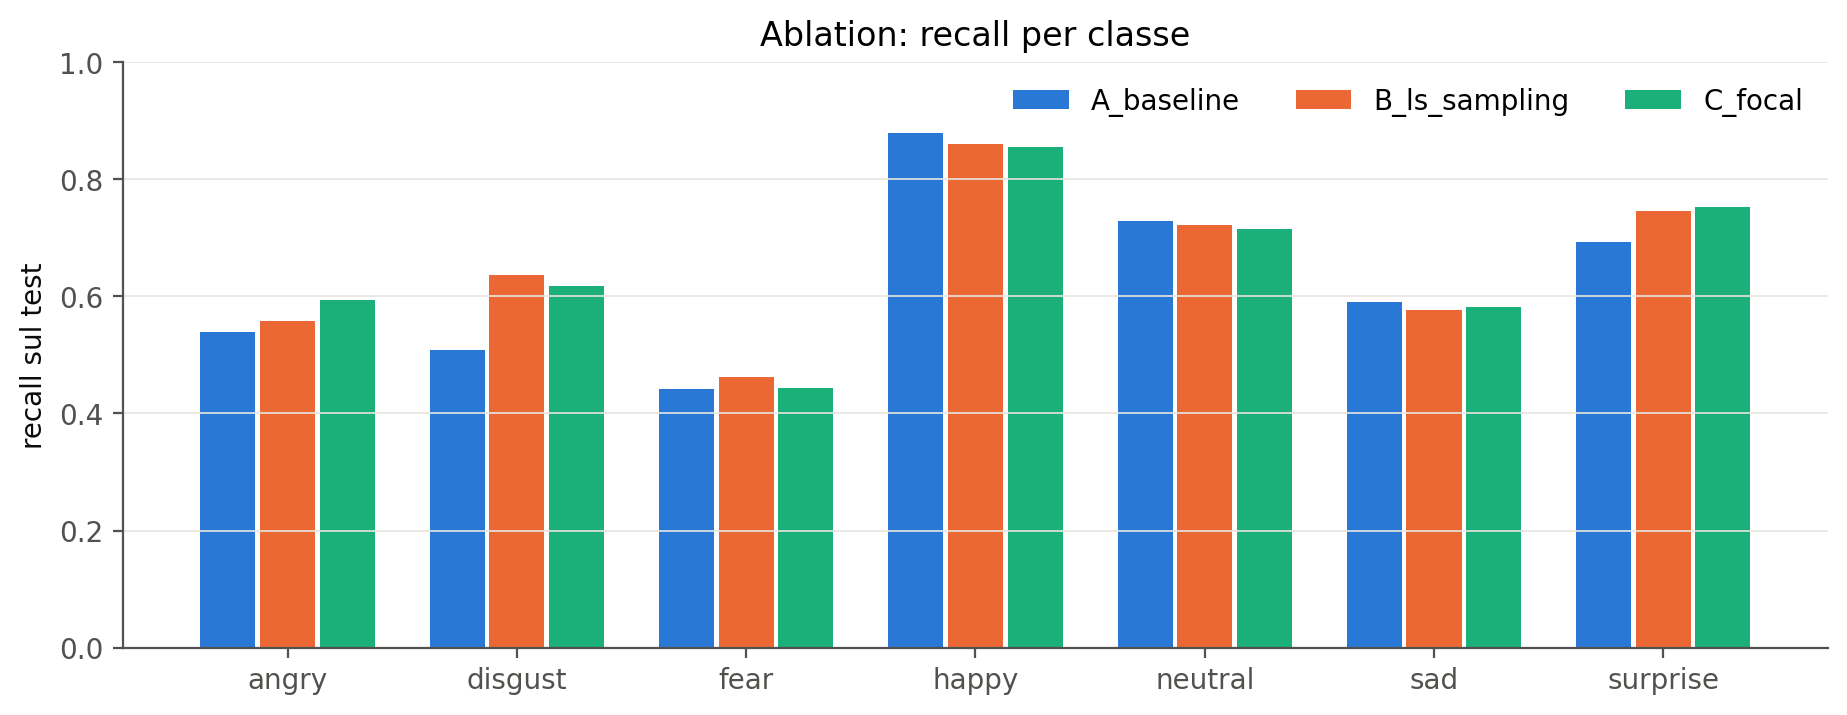
\includegraphics[width=\linewidth]{ablation_recall.png}
\caption{Ablation: recall per classe sul test delle tre configurazioni della ResNet-Lite.}
\label{fig:ablation}
\end{figure}

Le mitigazioni spostano il compromesso tra classi frequenti e rare: rispetto alla baseline, B e C aumentano la recall di \textit{Disgust}, \textit{Angry} e \textit{Surprise} e la riducono leggermente per \textit{Happy}. L'effetto netto è un aumento della macro-F1 di 1.5--2 punti senza variazioni significative dell'accuratezza. Il guadagno su \textit{Disgust} va interpretato con cautela: con soli 55 esempi di test, la recall di B (35/55, 0.636) ha un intervallo di confidenza di Wilson al 95\% di [0.50, 0.75], che si sovrappone a quello della baseline (28/55, 0.509, [0.38, 0.64]).

La SVM ottiene una recall di \textit{Disgust} relativamente alta (0.582) ma con una precisione di 0.110: i pesi di classe la spingono a predire \textit{Disgust} molto spesso, generando circa otto falsi positivi per ogni vero positivo.

\paragraph{Perché MobileNetV2 va peggio.} Il backbone congelato raggiunge solo il 40\% circa di accuratezza in validation: le feature apprese su foto a colori di ImageNet non sono direttamente adatte a volti $48\times48$ in scala di grigi. Il fine-tuning porta il modello al 62\% e la curva di validation si stabilizza nelle ultime epoche, quindi la differenza non dipende da un addestramento interrotto troppo presto. Il divario tra accuratezza di training (74.9\%) e di validation (61.9\%) è inoltre più ampio che per la ResNet-Lite (74.3\% contro 66.3\%): MobileNetV2 tende a memorizzare il training più che a generalizzare. L'ipotesi più probabile è la combinazione tra lo scarto di dominio e l'upscaling da 48 a 96 pixel, che non aggiunge informazione. Verificarla richiederebbe ulteriori esperimenti (ad esempio sbloccare l'intero backbone), non svolti per limiti di calcolo.

\section{Analisi critica: failure modes e bias}
\subsection{Matrice di confusione e classi simili}
\begin{figure}[H]
\centering
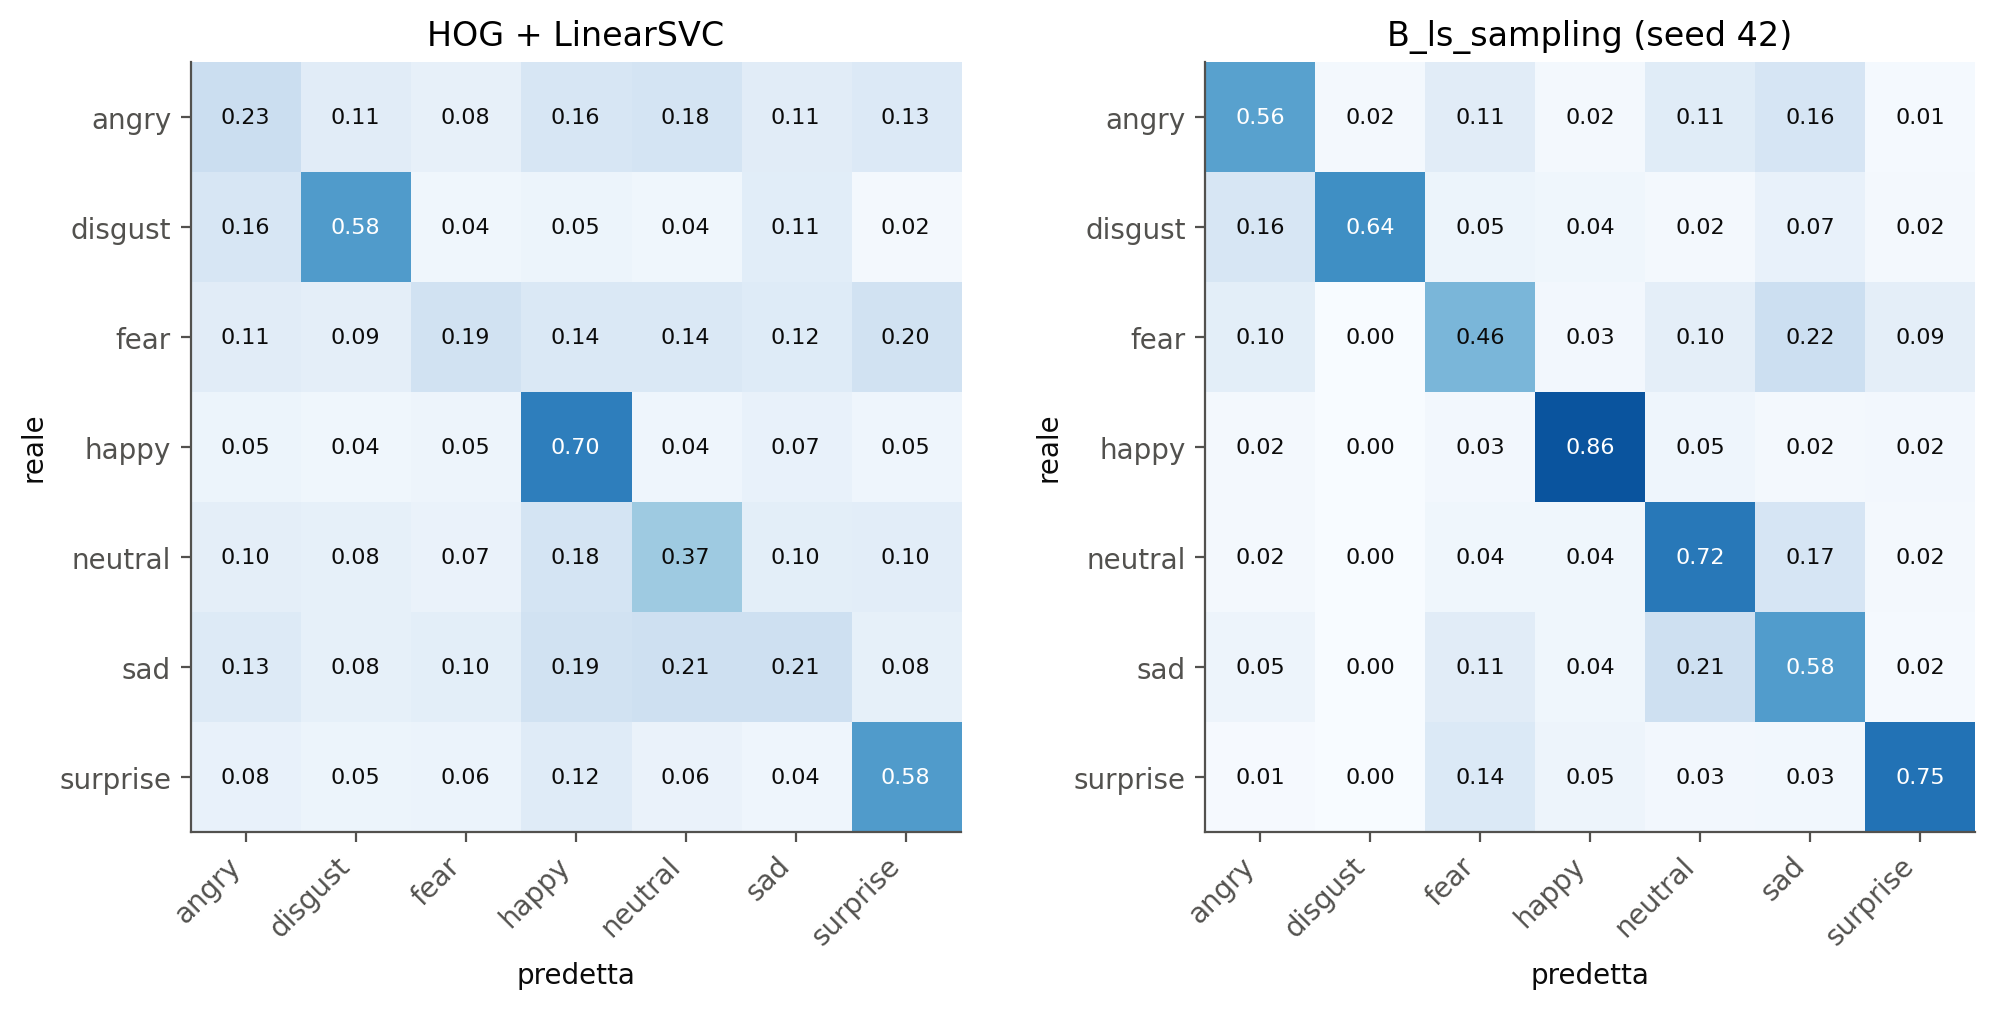
\includegraphics[width=\linewidth]{confusion_matrices.png}
\caption{Matrici di confusione normalizzate per riga sul test: HOG+LinearSVC (sinistra) e modello finale B (destra).}
\label{fig:cm}
\end{figure}

\begin{table}[H]
\centering
\caption{Precisione, recall e F1 per classe del modello finale (B, seed 42) sul test.}
\label{tab:perclass}
\begin{tabular}{lccccccc}
\toprule
 & Angry & Disgust & Fear & Happy & Neutral & Sad & Surprise \\
\midrule
Precisione & 0.695 & 0.673 & 0.517 & 0.891 & 0.616 & 0.506 & 0.758 \\
Recall     & 0.558 & 0.636 & 0.462 & 0.861 & 0.722 & 0.577 & 0.745 \\
F1         & 0.619 & 0.654 & 0.488 & 0.876 & 0.665 & 0.539 & 0.752 \\
\bottomrule
\end{tabular}
\end{table}

\textit{Happy} e \textit{Surprise} sono le classi più facili: sono caratterizzate da segni evidenti (sorriso, bocca e occhi spalancati) che restano visibili anche a $48\times48$. Le classi più difficili sono \textit{Fear} (F1 0.49) e \textit{Sad} (F1 0.54). Le confusioni più frequenti (reale $\rightarrow$ predetta) sono:
\begin{itemize}
    \item \textit{Fear} $\rightarrow$ \textit{Sad}: 21.6\% (114 immagini);
    \item \textit{Sad} $\rightarrow$ \textit{Neutral}: 20.5\% (122) e \textit{Neutral} $\rightarrow$ \textit{Sad}: 16.8\% (105);
    \item \textit{Angry} $\rightarrow$ \textit{Sad}: 16.5\% (81);
    \item \textit{Surprise} $\rightarrow$ \textit{Fear}: 13.7\% (57).
\end{itemize}
\textit{Sad} funziona da classe ``attrattore'' per le espressioni negative: \textit{Fear}, \textit{Angry} e \textit{Neutral} vi confluiscono quando i segnali distintivi sono deboli. La coppia \textit{Sad}--\textit{Neutral} è simmetrica: le due espressioni differiscono spesso solo per una lieve curvatura della bocca. La coppia \textit{Surprise}--\textit{Fear} condivide occhi spalancati e bocca aperta.

\subsection{Esempi di errore e rumore delle etichette}
\begin{figure}[H]
\centering
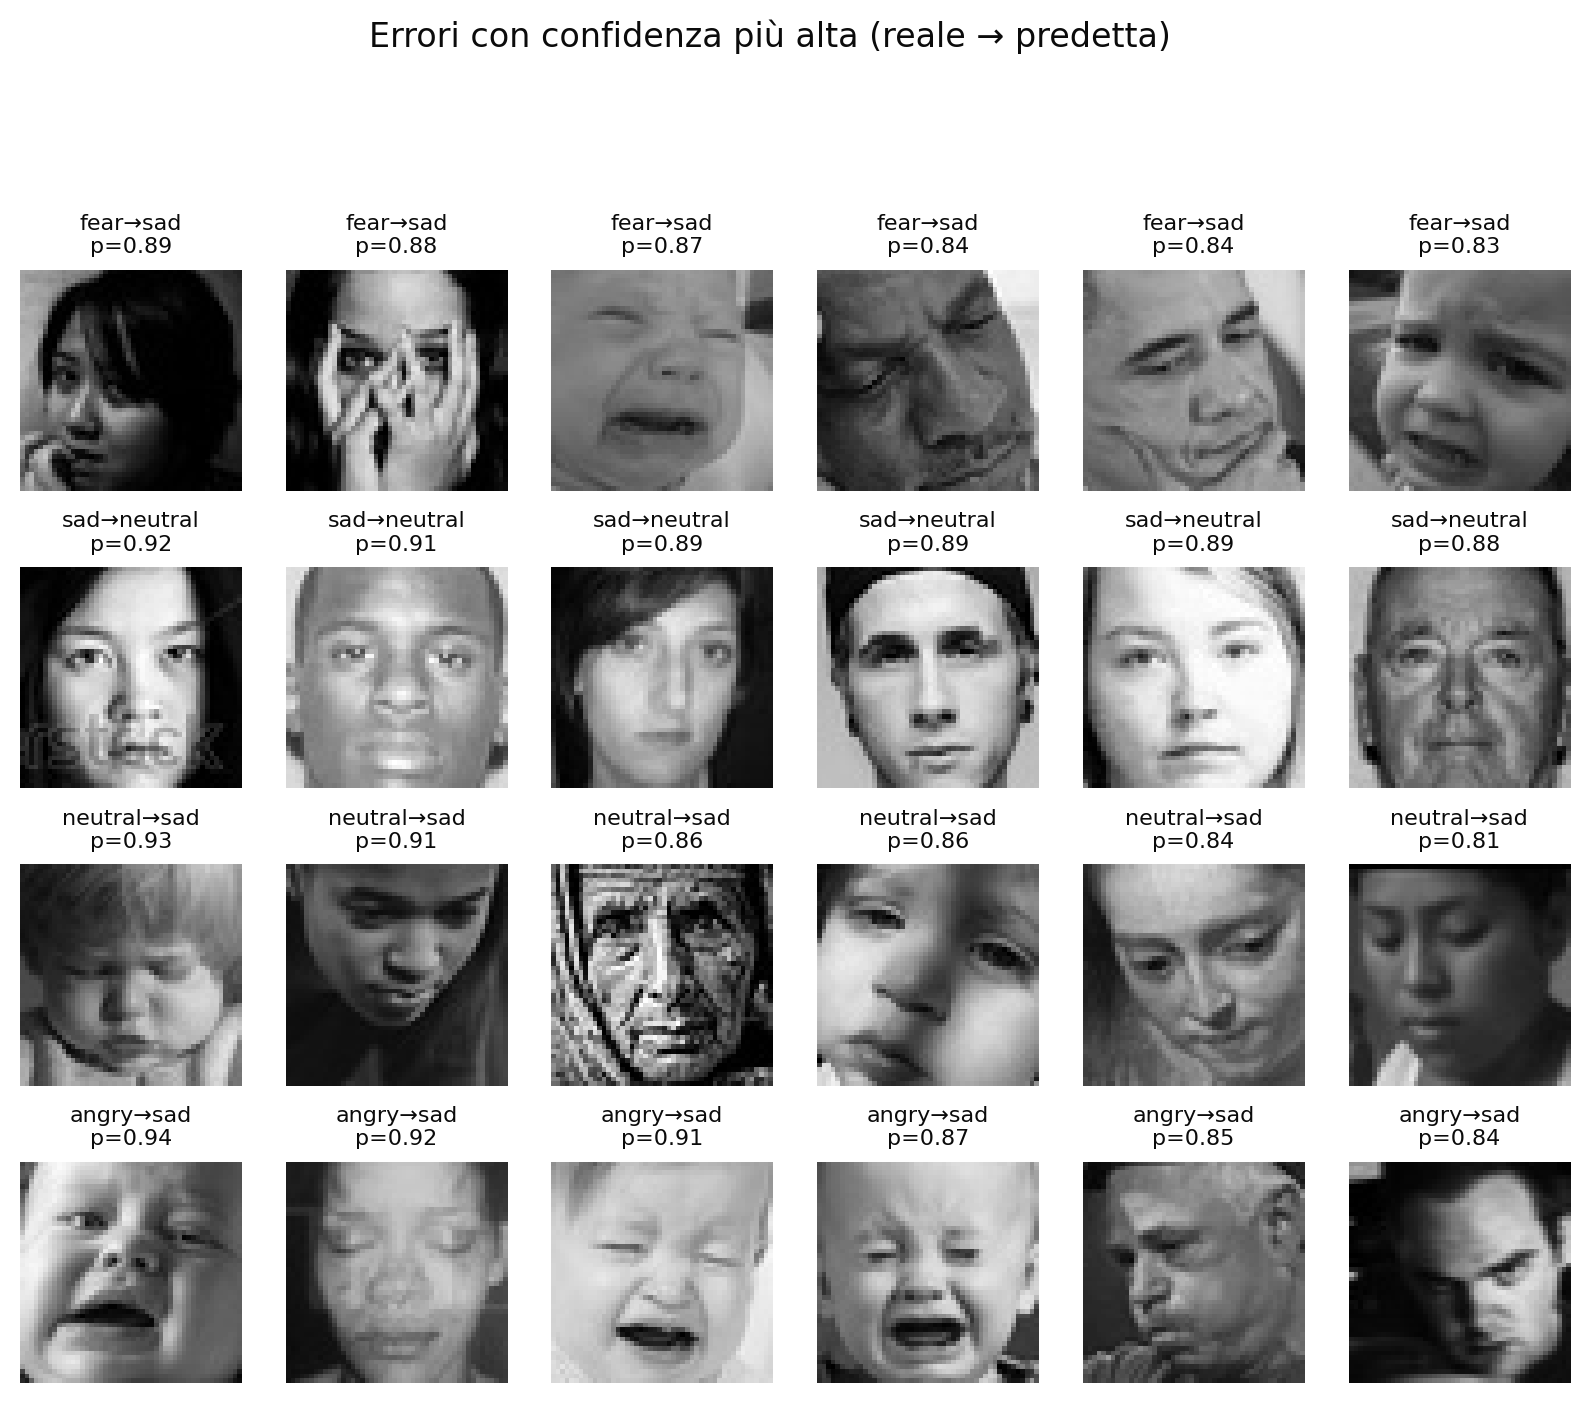
\includegraphics[width=0.85\linewidth]{failure_examples.png}
\caption{Errori del modello finale con la confidenza più alta, per le quattro coppie più confuse.}
\label{fig:failures}
\end{figure}

La Figura~\ref{fig:failures} mostra gli errori in cui il modello è più sicuro. Una parte di essi è difficile da considerare un errore del modello: diverse immagini etichettate \textit{Fear} o \textit{Angry} e predette \textit{Sad} ritraggono bambini in lacrime, e molti volti \textit{Sad} predetti \textit{Neutral} hanno un'espressione che un osservatore descriverebbe come neutra. Questo è coerente con il rumore di annotazione documentato per FER-2013 \cite{barsoum2016ferplus} e con le 57 immagini duplicate con etichette discordanti trovate nell'audit. Ne segue che una parte dell'errore residuo non è riducibile migliorando il modello, ma solo migliorando le etichette.

\subsection{Interpretabilità con Grad-CAM}
\begin{figure}[H]
\centering
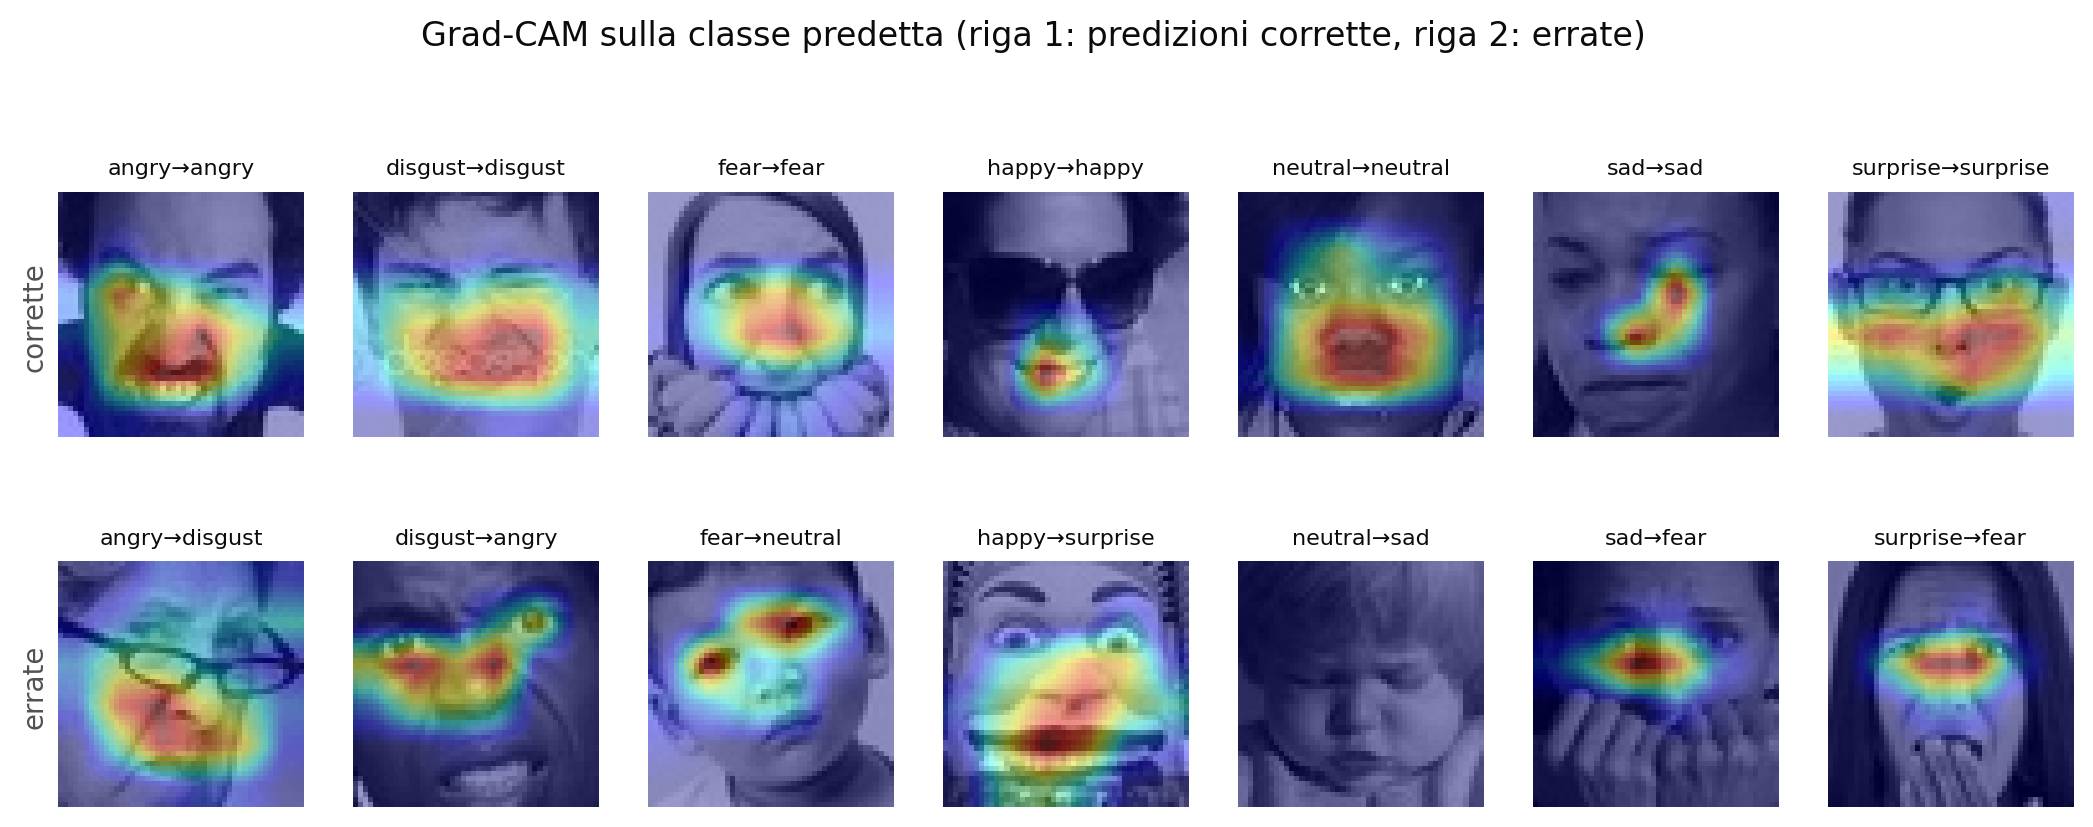
\includegraphics[width=\linewidth]{gradcam.png}
\caption{Mappe Grad-CAM sulla classe predetta: per ogni classe, un esempio corretto (sopra) e uno errato (sotto).}
\label{fig:gradcam}
\end{figure}

Grad-CAM \cite{selvaraju2017gradcam} evidenzia le regioni che più influenzano la predizione. Nelle predizioni corrette l'attivazione si concentra su bocca, naso e zona degli occhi, cioè le regioni che codificano le espressioni. Negli errori l'attivazione cade più spesso su elementi esterni o parziali: occhiali, mani davanti al volto, una sola regione del viso. Le mappe sono calcolate su una griglia $6\times6$ e vanno lette come indicazioni qualitative.

\subsection{Bias sui sottogruppi}
FER-2013 non contiene attributi demografici (genere, età, etnia): un'analisi demografica diretta non è possibile senza annotazioni aggiuntive. Stimare questi attributi con un altro modello su volti $48\times48$ introdurrebbe un errore difficile da controllare, che si sommerebbe a quello oggetto di studio. L'analisi si concentra quindi su tre fattori di acquisizione misurabili dai pixel: \textbf{luminosità} (media dei pixel), \textbf{contrasto} (deviazione standard) e \textbf{nitidezza} (varianza del Laplaciano). Per ciascun fattore il test set è diviso in quartili; si riportano accuratezza e \textit{balanced accuracy} (media delle recall per classe, che non dipende dalla composizione delle classi nel quartile), e si verifica l'indipendenza tra correttezza della predizione e quartile con un test del chi-quadro.

\begin{table}[H]
\centering
\caption{Accuratezza (balanced accuracy tra parentesi) del modello finale per quartile, dal valore più basso (Q1) al più alto (Q4). L'ultima colonna riporta il p-value del test del chi-quadro (3 gradi di libertà).}
\label{tab:bias}
\begin{tabular}{lccccc}
\toprule
Fattore & Q1 & Q2 & Q3 & Q4 & $p$ \\
\midrule
Luminosità & 64.8 (60.0) & 68.9 (66.1) & 65.9 (64.3) & 69.6 (65.6) & 0.085 \\
Contrasto  & 67.5 (63.5) & 68.6 (65.9) & 66.7 (64.0) & 66.5 (67.5) & 0.778 \\
Nitidezza  & 68.5 (64.2) & 66.0 (63.0) & 67.8 (64.2) & 66.9 (69.1) & 0.710 \\
\bottomrule
\end{tabular}
\end{table}

\begin{figure}[H]
\centering
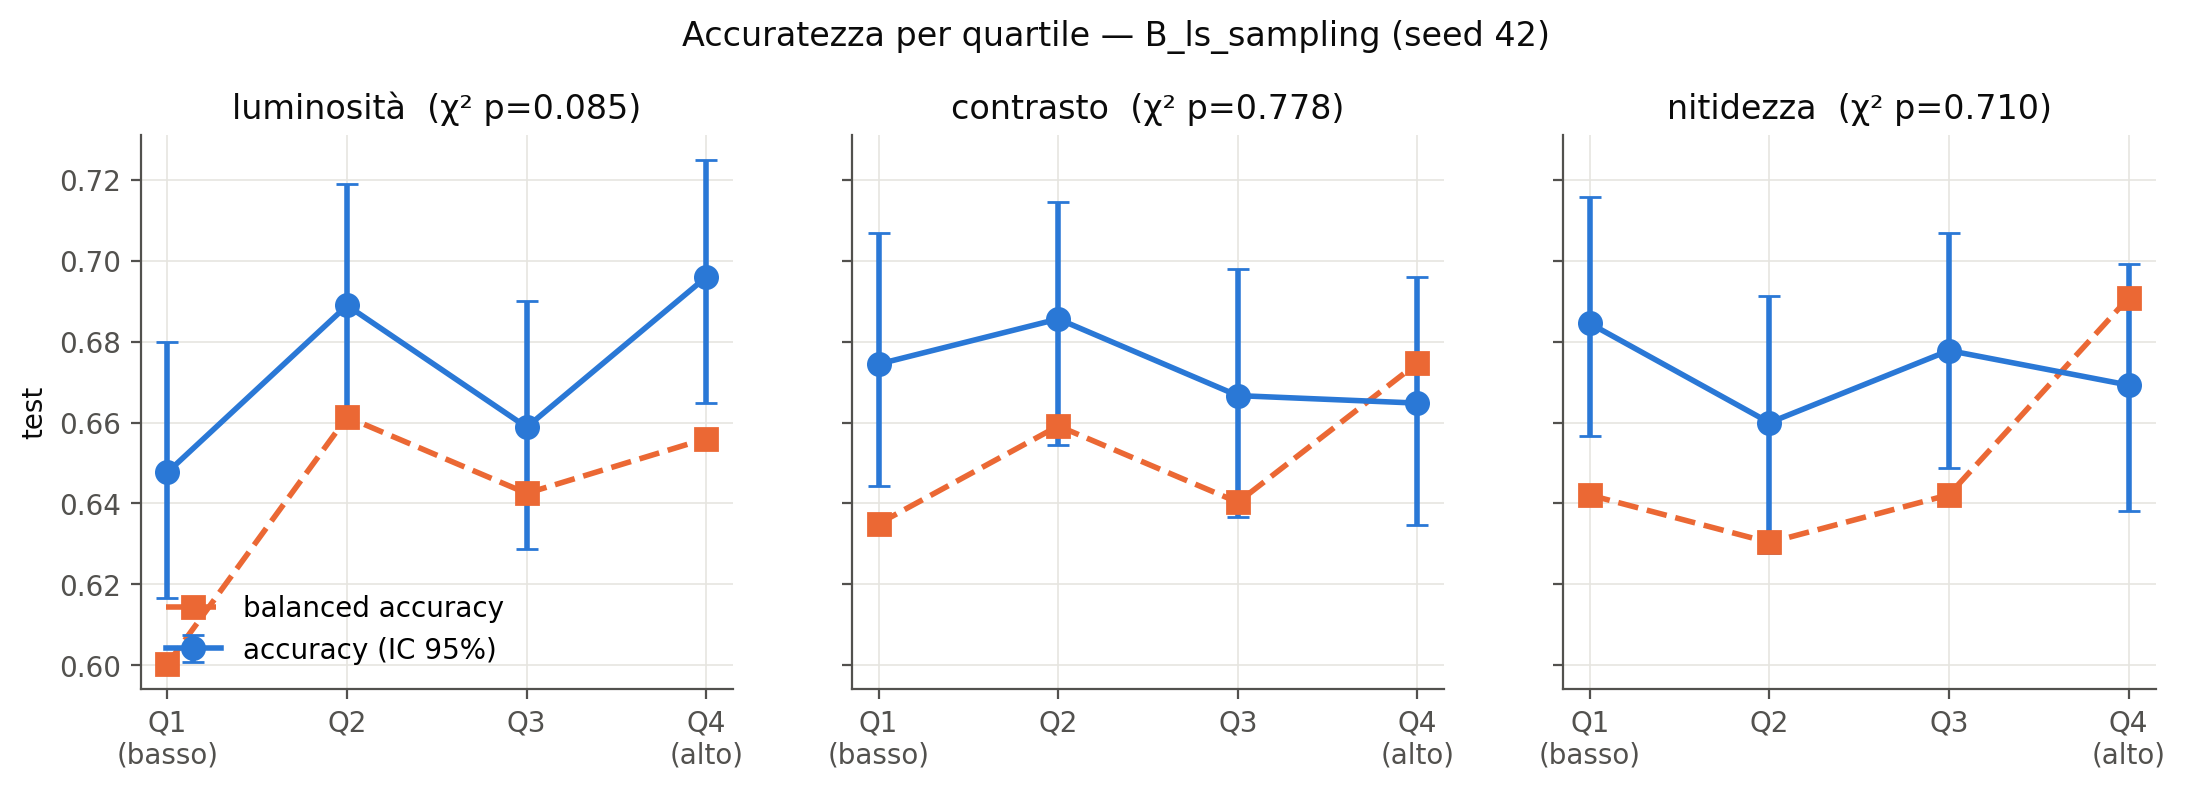
\includegraphics[width=\linewidth]{bias_subgroups.png}
\caption{Accuratezza (con IC bootstrap al 95\%) e balanced accuracy per quartile di luminosità, contrasto e nitidezza.}
\label{fig:bias}
\end{figure}

Contrasto e nitidezza non mostrano differenze apprezzabili. Per la luminosità, il quartile più scuro (intensità media inferiore a 106.6) ha l'accuratezza più bassa (64.8\% contro 69.6\% del quartile più chiaro) e anche la balanced accuracy più bassa (60.0\%). La differenza si ripete con tutti e tre i seed, ma non è statisticamente significativa al 5\% ($p=0.085$). Inoltre la distribuzione delle classi cambia molto tra i quartili di luminosità ($p\approx10^{-32}$): parte della differenza di accuratezza dipende da quali emozioni compaiono più spesso nelle immagini scure. Un'analisi esplorativa per classe mostra che il calo nel quartile più scuro si concentra su \textit{Fear} (recall 0.31 contro 0.57 nel quartile più chiaro) e \textit{Surprise} (0.60 contro 0.81), mentre \textit{Neutral} e \textit{Sad} vanno meglio al buio; questi confronti si basano su poche decine o centinaia di immagini per cella e non sono corretti per confronti multipli, quindi vanno letti come ipotesi. La conclusione corretta è quindi che esiste un'\textbf{evidenza debole} di prestazioni inferiori sulle immagini sottoesposte, da verificare con un test set più ampio; un $p$-value alto non dimostra l'assenza di un bias, indica solo che con questi dati non è rilevabile.

\section{Conclusioni}
\paragraph{Sintesi.} Su FER-2013, con un protocollo che separa validation e test e rimuove i duplicati tra split, una CNN residua compatta addestrata da zero raggiunge il $67.3\% \pm 0.2\%$ di accuratezza e una macro-F1 di 0.657, superando nettamente HOG+LinearSVC (40.6\%) e, in modo statisticamente significativo, MobileNetV2 in transfer learning (63.2\%). Il risultato è in linea con quanto riportato in letteratura per CNN singole addestrate senza dati aggiuntivi.

\paragraph{Mitigazioni.} Label smoothing e campionamento bilanciato non aumentano l'accuratezza globale, ma migliorano la macro-F1 e la recall delle classi rare. È il comportamento atteso: queste tecniche ridistribuiscono gli errori tra le classi invece di eliminarli.

\paragraph{Failure modes.} Gli errori si concentrano tra espressioni negative o poco marcate (\textit{Fear}, \textit{Sad}, \textit{Neutral}, \textit{Angry}). L'ispezione degli errori più sicuri suggerisce che una parte di essi è dovuta a etichette ambigue o errate.

\paragraph{Limiti.}
\begin{itemize}
    \item Ogni configurazione dell'ablation è stata addestrata con un solo seed; solo il modello finale è stato ripetuto su tre seed. Le differenze tra B e C sono inferiori alla variabilità attesa e non permettono di stabilire quale delle due mitigazioni sia migliore.
    \item La classe \textit{Disgust} ha solo 55 esempi di test: le sue metriche hanno intervalli di confidenza ampi.
    \item L'analisi dei bias è limitata a fattori di acquisizione: l'assenza di attributi demografici in FER-2013 impedisce di valutare l'equità rispetto a genere, età o etnia.
    \item Le etichette di FER-2013 sono rumorose: l'accuratezza misurata è una stima per difetto della capacità reale del modello di riconoscere le espressioni.
\end{itemize}

\paragraph{Sviluppi futuri.} Le direzioni più promettenti sono l'addestramento sulle etichette ri-annotate di FER+ \cite{barsoum2016ferplus}, che affronta direttamente il rumore; la valutazione su dataset con attributi demografici, per un'analisi di equità vera e propria \cite{xu2020bias}; la ripetizione dell'ablation su più seed per confrontare con significatività le strategie di mitigazione.

\bibliographystyle{unsrt}
\bibliography{references}

\end{document}
